\documentclass{scrartcl}

%\usepackage{algorithm}
%\usepackage{algorithmic}
\usepackage{amsmath}
\usepackage{amssymb}
%\usepackage{array}
%\usepackage{blindtext}
\usepackage{booktabs}
%\usepackage{colortbl}
%\usepackage{comment}
\usepackage{etex}
%\usepackage{float}
\usepackage[T1]{fontenc}
\usepackage{graphicx}
\usepackage[space]{grffile}
%\usepackage{multirow}
\usepackage[utf8]{inputenc}
\usepackage{pgfplots}
\usepackage{pgfplotstable}
\usepackage{morefloats}
\usepackage{subcaption}
%\usepackage{standalone}
\usepackage{times}
\usepackage{tikz}
%\usepackage{todonotes}
\usepackage{xspace}
\usepackage[breaklinks=true,colorlinks,bookmarks=false]{hyperref} %Hyperref should go last

%float setup
%\newfloat{algorithm}{t}{}
%
%%hyperref setup
\hypersetup{colorlinks=true}
\hypersetup{linktoc=all}
\hypersetup{draft=false}
\hypersetup{urlcolor=blue}
\hypersetup{citecolor=black}
\hypersetup{linkcolor=black}
%
%%tikz setup
%\usetikzlibrary{arrows,calc,external,fit,shapes}
\usetikzlibrary{external}
\tikzexternalize[prefix=ext/]
\tikzexternaldisable
%\usetikzlibrary{backgrounds}
%\usetikzlibrary{pgfplots.groupplots}
%
\pgfplotsset{compat=1.10}
%\pgfplotsset{filter discard warning=false}
%
%%Set graphics path
%\graphicspath{{figures//}}
%
%\DeclareMathOperator*{\argmin}{arg\,min}
%\DeclareMathOperator*{\argmax}{arg\,max}
%
%%Make require and ensure input and output
%\renewcommand{\algorithmicrequire}{\textbf{Input:}}
%\renewcommand{\algorithmicensure}{\textbf{Output:}}
%
%%This can be used to add external file dependencies for latexmk
%\makeatletter
%\newcommand*{\addFileDependency}[1]{% argument=file name and extension
%  \typeout{(#1)}% latexmk will find this if $recorder=0 (however, in that case, it will ignore #1 if it is a .aux or .pdf file etc and it exists! if it doesn't exist, it will appear in the list of dependents regardless)
%  \@addtofilelist{#1}% if you want it to appear in \listfiles, not really necessary and latexmk doesn't use this
%  \IfFileExists{#1}{}{\typeout{No file #1.}}% latexmk will find this message if #1 doesn't exist (yet)
%}
%\makeatother
%
\newcommand{\mytodo}[1]{\textcolor{red}{TODO: #1}}


\title{Machine Learning SS 2014}
\subtitle{Exercise Sheet 1}

\author{Georg Nebehay\\gnebehay@gmail.com}

\date{}

\tikzset{%
level 1/.style={sibling distance=10em},%
level 2/.style={sibling distance=7em},%
level 3/.style={sibling distance=3em}%
}

\begin{document}

\maketitle

\section{Decision Trees}

We modified the algorithm presented in the slides slightly in a sense that
a feature must not be selected in a node when it was already used in the previous node.


%\begin{table}[h!]
%  \centering
%  \begin{tabular}{cccccc|c}
%    \toprule
%    person      & eyes  & handsome & height & sex    & soccer & date\\
%    \midrule
%    Apu         & blue  & yes      & tall   & male   & no     & yes \\
%    Bernice     & brown & yes      & short  & female & no     & no  \\
%    Carl        & blue  & no       & tall   & male   & no     & yes \\
%    Doris       & green & yes      & short  & female & no     & no  \\
%    Edna        & brown & no       & short  & female & yes    & no  \\
%    Prof. Frink & brown & yes      & tall   & male   & yes    & no  \\
%    Gil         & blue  & no       & tall   & male   & yes    & no  \\
%    Homer       & green & yes      & short  & male   & no     & yes \\
%    Itchy       & brown & no       & short  & male   & yes    & yes \\
%    \bottomrule
%  \end{tabular}
%  \caption{Training data.}
%\end{table}

%\begin{table}[h!]
%  \centering
%  \begin{tabular}{cccccc|c}
%    \toprule
%    person      & eyes  & handsome & height & sex    & soccer & date\\
%    \midrule
%    Jimbo       & blue  & no       & tall   & male   & no     & yes\\
%    Krusty      & green & yes      & short  & male   & yes    & no\\
%    Lisa        & blue  & yes      & tall   & female & no     & no\\
%    Moe         & brown & no       & short  & male   & no     & no\\
%    Ned         & brown & yes      & short  & male   & no     & yes\\
%    Quimby      & blue  & no       & tall   & male   & no     & yes\\
%    \bottomrule
%  \end{tabular}
%  \caption{Test data.}
%\end{table}

\subsection{Without attribute ``soccer''}

At iteration 4, the algorithm enters an infinite recursion.
The problem stems from the omission of the soccer feature,
leading to the two datapoints Carl and Gil sharing exactly the same feature values but opposite labels.
We chose to stop the recursion at this point and to replace the node with the majority output of the parent node.
The grown decision tree is shown in Figure~\ref{fig:tree-nosoccer}.

\begin{figure}
\centering 
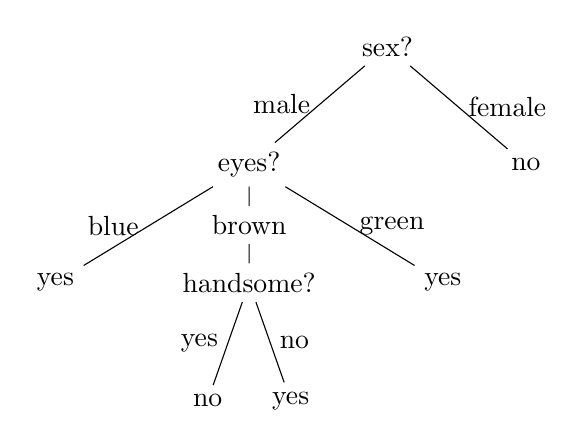
\begin{tikzpicture}
  \node {sex?}
  child { node {eyes?}
    child { node {yes} edge from parent node[left] {blue} }
    child { node {handsome?}
      child { node {no} edge from parent node[left] {yes} }
      child { node {yes} edge from parent node[right] {no} }
      edge from parent node[fill=white] {brown} }
    child { node {yes} edge from parent node[right] {green} }
    edge from parent node[left] {male} }
  child { node {no} 
    edge from parent node[right] {female}
  };
\end{tikzpicture}
\caption{Decision tree for task a)}
\label{fig:tree-nosoccer}
\end{figure}

\begin{table}[h!]
  \centering
  \begin{tabular}{cccccc|c|c}
    \toprule
    person      & eyes  & handsome & height & sex    & soccer & date & tree\\
    \midrule
    Jimbo       & blue  & no       & tall   & male   & no     & yes & yes\\
    Krusty      & green & yes      & short  & male   & yes    & no  & yes\\
    Lisa        & blue  & yes      & tall   & female & no     & no  & no\\
    Moe         & brown & no       & short  & male   & no     & no  & yes\\
    Ned         & brown & yes      & short  & male   & no     & yes & no\\
    Quimby      & blue  & no       & tall   & male   & no     & yes & yes\\
    \bottomrule
  \end{tabular}
  \caption{Classification result for tree a) on the test set. Accuracy is 3/6.}
\end{table}


\subsection{Without attribute ``eyecolor''}

The decision tree is shown in Figure~\ref{fig:tree-noeyes}.

\begin{figure}
\centering 
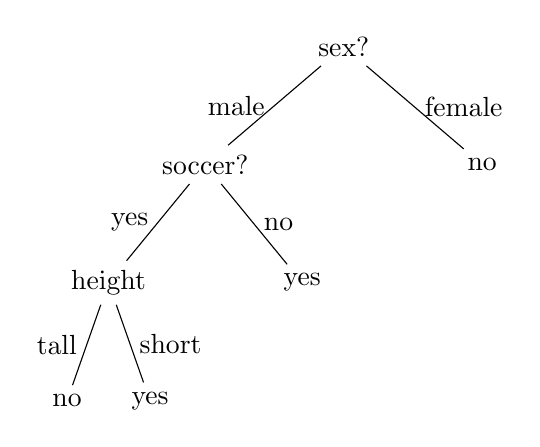
\begin{tikzpicture}
  \node {sex?}
  child { node {soccer?}
    child { node {height}
    child { node {no} edge from parent node[left] {tall} }
    child { node {yes} edge from parent node[right] {short} }
      edge from parent node[left] {yes} }
    child { node {yes} edge from parent node[right] {no} }
    edge from parent node[left] {male} }
  child { node {no} 
    edge from parent node[right] {female}
  };
\end{tikzpicture}
\caption{Decision tree for task b)}
\label{fig:tree-noeyes}
\end{figure}

\begin{table}[h!]
  \centering
  \begin{tabular}{cccccc|c|c}
    \toprule
    person      & eyes  & handsome & height & sex    & soccer & date & tree\\
    \midrule
    Jimbo       & blue  & no       & tall   & male   & no     & yes & yes\\
    Krusty      & green & yes      & short  & male   & yes    & no  & yes\\
    Lisa        & blue  & yes      & tall   & female & no     & no  & no \\
    Moe         & brown & no       & short  & male   & no     & no  & yes\\
    Ned         & brown & yes      & short  & male   & no     & yes & yes\\
    Quimby      & blue  & no       & tall   & male   & no     & yes & yes\\
    \bottomrule
  \end{tabular}
  \caption{Classification result for tree b) on the test set. Accuracy is 4/6.}
\end{table}

\subsection{Itchy has label ``no''}

The decision tree is shown in Figure~\ref{fig:tree-itchyno}.

\begin{figure}
\centering 
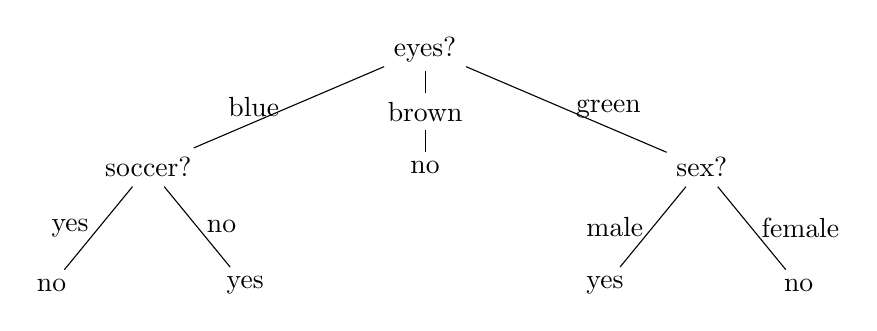
\begin{tikzpicture}
\node {eyes?}
  child { node {soccer?}
    child { node {no} edge from parent node[left] {yes} }
    child { node {yes} edge from parent node[right] {no} }
    edge from parent node[left] {blue} }
  child { node {no} edge from parent node[fill=white] {brown} }
  child { node {sex?}
    child { node {yes} edge from parent node[left] {male} }
    child { node {no} edge from parent node[right] {female} }
  edge from parent node[right] {green} }
;
\end{tikzpicture}
\caption{Decision tree for task c)}
\label{fig:tree-itchyno}
\end{figure}

\begin{table}[h!]
  \centering
  \begin{tabular}{cccccc|c|c}
    \toprule
    person      & eyes  & handsome & height & sex    & soccer & date & tree\\
    \midrule
    Jimbo       & blue  & no       & tall   & male   & no     & yes & no \\
    Krusty      & green & yes      & short  & male   & yes    & no  & yes\\
    Lisa        & blue  & yes      & tall   & female & no     & no  & yes\\
    Moe         & brown & no       & short  & male   & no     & no  & no \\
    Ned         & brown & yes      & short  & male   & no     & yes & no \\
    Quimby      & blue  & no       & tall   & male   & no     & yes & yes\\
    \bottomrule
  \end{tabular}
  \caption{Classification result for tree c) on the test set. Accuracy is 2/6.}
\end{table}

\subsection{Additional training example ``Ralph''}

The decision tree is shown in Figure~\ref{fig:tree-ralph}.

\begin{figure}
\centering 
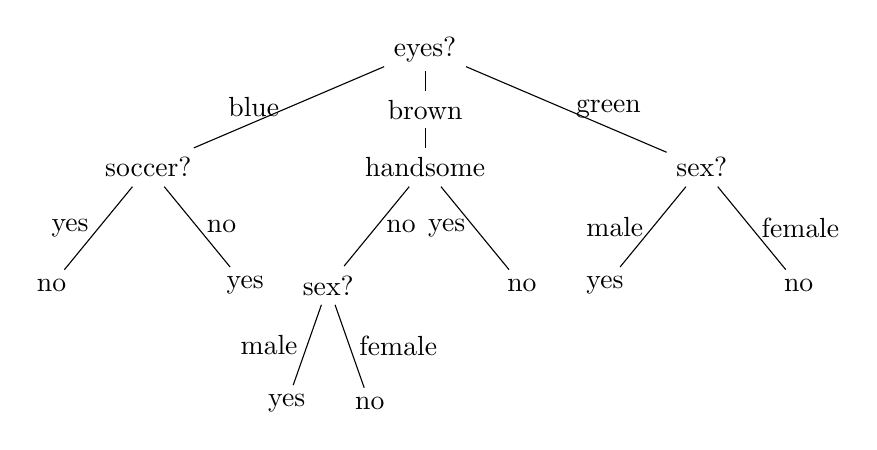
\begin{tikzpicture}
\node {eyes?}
  child { node {soccer?}
    child { node {no} edge from parent node[left] {yes} }
    child { node {yes} edge from parent node[right] {no} }
    edge from parent node[left] {blue} }
  child { node {handsome}
    child { node {sex?}
      child { node {yes} edge from parent node[left] {male} }
      child { node {no} edge from parent node[right] {female} }
      edge from parent node[right] {no} }
    child { node {no} edge from parent node[left] {yes} }
    edge from parent node[fill=white] {brown} }
  child { node {sex?}
    child { node {yes} edge from parent node[left] {male} }
    child { node {no} edge from parent node[right] {female} }
    edge from parent node[right] {green} }
;
\end{tikzpicture}
\caption{Decision tree for task d)}
\label{fig:tree-ralph}
\end{figure}

\begin{table}[h!]
  \centering
  \begin{tabular}{cccccc|c|c}
    \toprule
    person      & eyes  & handsome & height & sex    & soccer & date & tree\\
    \midrule
    Jimbo       & blue  & no       & tall   & male   & no     & yes & yes\\
    Krusty      & green & yes      & short  & male   & yes    & no  & yes\\
    Lisa        & blue  & yes      & tall   & female & no     & no  & yes\\
    Moe         & brown & no       & short  & male   & no     & no  & yes\\
    Ned         & brown & yes      & short  & male   & no     & yes & no \\
    Quimby      & blue  & no       & tall   & male   & no     & yes & yes\\
    \bottomrule
  \end{tabular}
  \caption{Classification result for tree d) on the test set. Accuracy is 2/6.}
\end{table}

\section{Nearest Neighbour Classification}
\section{Capacity \& Overfitting}
\section{Missing Proofs}
\section{Practical Experiments I}
\section{Practical Experiments II}

\begin{appendix}
\begin{table}[h!]
  \centering
  \begin{tabular}{ccccc|c}
    \toprule
    person      & eyes  & handsome & height & sex    & date\\
    \midrule
    Apu         & blue  & yes      & tall   & male   & yes \\
    Bernice     & brown & yes      & short  & female & no  \\
    Carl        & blue  & no       & tall   & male   & yes \\
    Doris       & green & yes      & short  & female & no  \\
    Edna        & brown & no       & short  & female & no  \\
    Prof. Frink & brown & yes      & tall   & male   & no  \\
    Gil         & blue  & no       & tall   & male   & no  \\
    Homer       & green & yes      & short  & male   & yes \\
    Itchy       & brown & no       & short  & male   & yes \\
    \bottomrule
  \end{tabular}

  \vspace{.5cm}

  \begin{tabular}{ccc}
    \toprule
    Feature      & Accuracies                              & Total\\
    \midrule
    eyes         & blue: (2/3), brown: (3/4), green: (1/2) & 6/9\\
    handsome     & yes: (3/5), no: (2/4)                   & 5/9\\
    height       & tall: (2/4), short: (3/5)               & 5/9\\
    \textbf{sex} & male: (4/6), female: (3/3) [no]         & \textbf{7/9}\\
    \bottomrule
  \end{tabular}
  \caption*{No soccer, iteration 1, root branch. Best feature: sex}
\end{table}

\begin{table}[h!]
  \centering
  \begin{tabular}{ccccc|c}
    \toprule
    person      & eyes  & handsome & height & sex    & date\\
    \midrule
    Apu         & blue  & yes      & tall   & male   & yes \\
    Carl        & blue  & no       & tall   & male   & yes \\
    Prof. Frink & brown & yes      & tall   & male   & no  \\
    Gil         & blue  & no       & tall   & male   & no  \\
    Homer       & green & yes      & short  & male   & yes \\
    Itchy       & brown & no       & short  & male   & yes \\
    \bottomrule
  \end{tabular}

  \vspace{.5cm}

  \begin{tabular}{ccc}
    \toprule
    Feature       & Accuracies                                    & Total\\
    \midrule
    \textbf{eyes} & blue: (2/3), brown: (1/2), green: (1/1) [yes] & 4/6\\
    handsome      & yes: (2/3), no: (2/3)                         & 4/6\\
    height        & tall: (2/4), short: (2/2)                     & 4/6\\
    sex           & male: (4/6)                                   & 4/6\\
    \bottomrule
  \end{tabular}
  \caption*{No soccer, iteration 2, sex=male branch. Best feature: eyes}
\end{table}

\begin{table}[h!]
  \centering
  \begin{tabular}{ccccc|c}
    \toprule
    person      & eyes  & handsome & height & sex    & date\\
    \midrule
    Apu         & blue  & yes      & tall   & male   & yes \\
    Carl        & blue  & no       & tall   & male   & yes \\
    Gil         & blue  & no       & tall   & male   & no  \\
    \bottomrule
  \end{tabular}

  \vspace{.5cm}

  \begin{tabular}{ccc}
    \toprule
    Feature           & Accuracies                  & Total\\
    \midrule
    eyes              & blue: (2/3)                 & \textbf{2/3}\\
    \textbf{handsome} & yes: (1/1) [yes], no: (1/2) & \textbf{2/3}\\
    height            & tall: (2/3)                 & \textbf{2/3}\\
    sex               & male: (2/3)                 & \textbf{2/3}\\
    \bottomrule
  \end{tabular}
  \caption*{No soccer, iteration 3, sex=male,eyes/blue branch. Best feature: handsome}
\end{table}

\begin{table}[h!]
  \centering
  \begin{tabular}{ccccc|c}
    \toprule
    person      & eyes  & handsome & height & sex    & date\\
    \midrule
    Carl        & blue  & no       & tall   & male   & yes \\
    Gil         & blue  & no       & tall   & male   & no  \\
    \bottomrule
  \end{tabular}

  \vspace{.5cm}

  \begin{tabular}{ccc}
    \toprule
    Feature           & Accuracies                  & Total\\
    \midrule
    eyes              & blue: (1/2)                 & 1/2\\
    handsome          & no: (1/2)                   & 1/2\\
    height            & tall: (1/2)                 & 1/2\\
    sex               & male: (1/2)                 & 1/2\\
    \bottomrule
  \end{tabular}
  \caption*{No soccer, iteration 4, sex=male,eyes/blue,handsome=no branch.
  Stopping because of infinite recursion that lies ahead.}
\end{table}

\begin{table}[h!]
  \centering
  \begin{tabular}{ccccc|c}
    \toprule
    person      & eyes  & handsome & height & sex    & date\\
    \midrule
    Prof. Frink & brown & yes      & tall   & male   & no  \\
    Itchy       & brown & no       & short  & male   & yes \\
    \bottomrule
  \end{tabular}

  \vspace{.5cm}

  \begin{tabular}{ccc}
    \toprule
    Feature           & Accuracies                              & Total\\
    \midrule
    eyes              & brown: (1/2)                            & 1/2\\
    \textbf{handsome} & yes: (1/1) [no], no: (1/1) [yes]        & \textbf{2/2}\\
    height            & tall: (1/1), short: (1/1)               & \textbf{2/2}\\
    sex               & male: (1/2)                             & 1/2\\
    \bottomrule
  \end{tabular}
  \caption*{No soccer, iteration 5, sex=male,eyes=brown branch. Best feature: handsome}
\end{table}


\begin{table}[h!]
  \centering
  \begin{tabular}{ccccc|c}
    \toprule
    person      & handsome & height & sex    & soccer & date\\
    \midrule
    Apu         & yes      & tall   & male   & no     & yes \\
    Bernice     & yes      & short  & female & no     & no  \\
    Carl        & no       & tall   & male   & no     & yes \\
    Doris       & yes      & short  & female & no     & no  \\
    Edna        & no       & short  & female & yes    & no  \\
    Prof. Frink & yes      & tall   & male   & yes    & no  \\
    Gil         & no       & tall   & male   & yes    & no  \\
    Homer       & yes      & short  & male   & no     & yes \\
    Itchy       & no       & short  & male   & yes    & yes \\
    \bottomrule
  \end{tabular}

  \vspace{.5cm}

  \begin{tabular}{ccc}
    \toprule
    Feature      & Accuracies                              & Total\\
    \midrule
    handsome     & yes: (3/5), no: (2/4)                   & 5/9\\
    height       & tall: (2/4), short: (3/5)               & 5/9\\
    \textbf{sex} & male: (4/6), female: (3/3) [no]         & \textbf{7/9}\\
    soccer       & yes: (3/4), no: (3/5)                   & 6/9\\
    \bottomrule
  \end{tabular}
  \caption*{No eyes, iteration 1, root branch. Best feature: sex}
\end{table}

\begin{table}[h!]
  \centering
  \begin{tabular}{ccccc|c}
    \toprule
    person      & handsome & height & sex    & soccer & date\\
    \midrule
    Apu         & yes      & tall   & male   & no     & yes \\
    Carl        & no       & tall   & male   & no     & yes \\
    Prof. Frink & yes      & tall   & male   & yes    & no  \\
    Gil         & no       & tall   & male   & yes    & no  \\
    Homer       & yes      & short  & male   & no     & yes \\
    Itchy       & no       & short  & male   & yes    & yes \\
    \bottomrule
  \end{tabular}

  \vspace{.5cm}

  \begin{tabular}{ccc}
    \toprule
    Feature         & Accuracies                              & Total\\
    \midrule
    handsome        & yes: (2/3), no: (2/3)                   & 4/6\\
    height          & tall: (2/4), short: (2/2)               & 4/6\\
    sex             & male: (4/6)                             & 4/6\\
    \textbf{soccer} & yes: (2/3), no: (3/3) [yes]             & \textbf{5/6}\\
    \bottomrule
  \end{tabular}
  \caption*{No eyes, iteration 2, sex/male branch. Best feature: soccer}
\end{table}

\begin{table}[h!]
  \centering
  \begin{tabular}{ccccc|c}
    \toprule
    person      & handsome & height & sex    & soccer & date\\
    \midrule
    Prof. Frink & yes      & tall   & male   & yes    & no  \\
    Gil         & no       & tall   & male   & yes    & no  \\
    Itchy       & no       & short  & male   & yes    & yes \\
    \bottomrule
  \end{tabular}

  \vspace{.5cm}

  \begin{tabular}{ccc}
    \toprule
    Feature         & Accuracies                              & Total\\
    \midrule
    handsome        & yes: (1/1), no: (1/2)                   & 2/3\\
    \textbf{height} & tall: (2/2) [no], short: (1/1) [yes]    & \textbf{3/3}\\
    sex             & male: (2/3)                             & 2/3\\
    soccer          & yes: (2/3)                              & 2/3\\
    \bottomrule
  \end{tabular}
  \caption*{No eyes, iteration 3, soccer/yes branch. Best feature: height}
\end{table}

\begin{table}[h!]
  \centering
  \begin{tabular}{cccccc|c}
    \toprule
    person      & eyes  & handsome & height & sex    & soccer & date\\
    \midrule
    Apu         & blue  & yes      & tall   & male   & no     & yes \\
    Bernice     & brown & yes      & short  & female & no     & no  \\
    Carl        & blue  & no       & tall   & male   & no     & yes \\
    Doris       & green & yes      & short  & female & no     & no  \\
    Edna        & brown & no       & short  & female & yes    & no  \\
    Prof. Frink & brown & yes      & tall   & male   & yes    & no  \\
    Gil         & blue  & no       & tall   & male   & yes    & no  \\
    Homer       & green & yes      & short  & male   & no     & yes \\
    Itchy       & brown & no       & short  & male   & yes    & no  \\
    \bottomrule
  \end{tabular}

  \vspace{.5cm}

  \begin{tabular}{ccc}
    \toprule
    Feature      & Accuracies                                    & Total\\
    \midrule
    \textbf{eyes} & blue: (2/3), brown: (4/4) [no], green: (1/2) & \textbf{7/9}\\
    handsome      & yes: (3/5), no: (3/4)                        & 6/9\\
    height        & tall: (2/4), short: (4/5)                    & 6/9\\
    sex           & male: (3/6), female: (3/3)                   & 6/9\\
    soccer        & yes: (4/4), no: (3/5)                        & \textbf{7/9}\\
    \bottomrule
  \end{tabular}
  \caption*{Itchy no, iteration 1, root branch. Best feature: eyes}
\end{table}

\begin{table}[h!]
  \centering
  \begin{tabular}{cccccc|c}
    \toprule
    person      & eyes  & handsome & height & sex    & soccer & date\\
    \midrule
    Apu         & blue  & yes      & tall   & male   & no     & yes \\
    Carl        & blue  & no       & tall   & male   & no     & yes \\
    Gil         & blue  & no       & tall   & male   & yes    & no  \\
    \bottomrule
  \end{tabular}

  \vspace{.5cm}

  \begin{tabular}{ccc}
    \toprule
    Feature         & Accuracies                              & Total\\
    \midrule
    eyes            & blue: (2/3)                             & 2/3\\
    handsome        & yes: (1/1), no: (1/2)                   & 2/3\\
    height          & tall: (2/3)                             & 2/3\\
    sex             & male: (2/3)                             & 2/3\\
    \textbf{soccer} & yes: (1/1) [no], no: (2/2) [yes]        & \textbf{3/3}\\
    \bottomrule
  \end{tabular}
  \caption*{Itchy no, iteration 2, eyes=blue branch. Best feature: soccer}
\end{table}

\begin{table}[h!]
  \centering
  \begin{tabular}{cccccc|c}
    \toprule
    person      & eyes  & handsome & height & sex    & soccer & date\\
    \midrule
    Doris       & green & yes      & short  & female & no     & no  \\
    Homer       & green & yes      & short  & male   & no     & yes \\
    \bottomrule
  \end{tabular}

  \vspace{.5cm}

  \begin{tabular}{ccc}
    \toprule
    Feature      & Accuracies                              & Total\\
    \midrule
    eyes         & green: (1/2)                            & 1/2\\
    handsome     & yes: (1/2)                              & 1/2\\
    height       & short: (1/2)                            & 1/2\\
    \textbf{sex} & male: (1/1) [yes], female: (1/1) [no]   & \textbf{2/2}\\
    soccer       & no: (1/2)                               & 7/9\\
    \bottomrule
  \end{tabular}
  \caption*{Itchy no, iteration 3, eyes=green branch. Best feature: sex}
\end{table}

\begin{table}[h!]
  \centering
  \begin{tabular}{cccccc|c}
    \toprule
    person      & eyes  & handsome & height & sex    & soccer & date\\
    \midrule
    Apu         & blue  & yes      & tall   & male   & no     & yes \\
    Bernice     & brown & yes      & short  & female & no     & no  \\
    Carl        & blue  & no       & tall   & male   & no     & yes \\
    Doris       & green & yes      & short  & female & no     & no  \\
    Edna        & brown & no       & short  & female & yes    & no  \\
    Prof. Frink & brown & yes      & tall   & male   & yes    & no  \\
    Gil         & blue  & no       & tall   & male   & yes    & no  \\
    Homer       & green & yes      & short  & male   & no     & yes \\
    Itchy       & brown & no       & short  & male   & yes    & yes \\
    Ralph       & green & no       & short  & male   & yes    & no  \\
    \bottomrule
  \end{tabular}

  \vspace{.5cm}

  \begin{tabular}{ccc}
    \toprule
    Feature         & Accuracies                              & Total\\
    \midrule
    \textbf{eyes}   & blue: (2/3), brown: (3/4), green: (2/3) & \textbf{7/10}\\
    handsome        & yes: (3/5), no: (3/5)                   & 6/10\\
    height          & tall: (2/4), short: (4/6)               & 6/10\\
    sex             & male: (4/7), female: (3/3)              & \textbf{7/10}\\
    soccer          & yes: (4/5), no: (3/5)                   & \textbf{7/10}\\
    \bottomrule
  \end{tabular}
  \caption*{Ralph, iteration 1, root branch. Best feature: eyes}
\end{table}

\begin{table}[h!]
  \centering
  \begin{tabular}{cccccc|c}
    \toprule
    person      & eyes  & handsome & height & sex    & soccer & date\\
    \midrule
    Apu         & blue  & yes      & tall   & male   & no     & yes \\
    Carl        & blue  & no       & tall   & male   & no     & yes \\
    Gil         & blue  & no       & tall   & male   & yes    & no  \\
    \bottomrule
  \end{tabular}

  \vspace{.5cm}

  \begin{tabular}{ccc}
    \toprule
    Feature         & Accuracies                              & Total\\
    \midrule
    eyes            & blue: (2/3)                             & 2/3\\
    handsome        & yes: (1/1), no: (1/2)                   & 2/3\\
    height          & tall: (2/3)                             & 2/3\\
    sex             & male: (2/3)                             & 2/3\\
    \textbf{soccer} & yes: (1/1) [no], no: (2/2) [yes]        & \textbf{3/3}\\
    \bottomrule
  \end{tabular}
  \caption*{Ralph, iteration 2, eyes=blue branch. Best feature: soccer}
\end{table}

\begin{table}[h!]
  \centering
  \begin{tabular}{cccccc|c}
    \toprule
    person      & eyes  & handsome & height & sex    & soccer & date\\
    \midrule
    Bernice     & brown & yes      & short  & female & no     & no  \\
    Edna        & brown & no       & short  & female & yes    & no  \\
    Prof. Frink & brown & yes      & tall   & male   & yes    & no  \\
    Itchy       & brown & no       & short  & male   & yes    & yes \\
    \bottomrule
  \end{tabular}

  \vspace{.5cm}

  \begin{tabular}{ccc}
    \toprule
    Feature           & Accuracies                              & Total\\
    \midrule
    eyes              & brown: (3/4)                            & \textbf{3/4}\\
    \textbf{handsome} & yes: (2/2) [no], no: (1/2)              & \textbf{3/4}\\
    height            & tall: (1/1), short: (2/3)               & \textbf{3/4}\\
    sex               & male: (1/2), female: (2/2)              & \textbf{3/4}\\
    soccer            & yes: (2/3), no: (1/1)                   & \textbf{3/4}\\
    \bottomrule
  \end{tabular}
  \caption*{Ralph, iteration 3, eyes=brown branch. Best feature: handsome}
\end{table}

\begin{table}[h!]
  \centering
  \begin{tabular}{cccccc|c}
    \toprule
    person      & eyes  & handsome & height & sex    & soccer & date\\
    \midrule
    Edna        & brown & no       & short  & female & yes    & no  \\
    Itchy       & brown & no       & short  & male   & yes    & yes \\
    \bottomrule
  \end{tabular}

  \vspace{.5cm}

  \begin{tabular}{ccc}
    \toprule
    Feature           & Accuracies                            & Total\\
    \midrule
    eyes              & brown: (1/2)                          & 1/2\\
    handsome          & no: (1/2)                             & 1/2\\
    height            & short: (1/2)                          & 1/2\\
    \textbf{sex}      & male: (1/1) [yes], female: (1/1) [no] & 2/2\\
    soccer            & yes: (1/2)                            & 1/2\\
    \bottomrule
  \end{tabular}
  \caption*{Ralph, iteration 4, eyes=brown,handsome=no branch. Best feature: sex}
\end{table}

\begin{table}[h!]
  \centering
  \begin{tabular}{cccccc|c}
    \toprule
    person      & eyes  & handsome & height & sex    & soccer & date\\
    \midrule
    Doris       & green & yes      & short  & female & no     & no  \\
    Homer       & green & yes      & short  & male   & no     & yes \\
    Ralph       & green & no       & short  & male   & yes    & no  \\
    \bottomrule
  \end{tabular}

  \vspace{.5cm}

  \begin{tabular}{ccc}
    \toprule
    Feature           & Accuracies                              & Total\\
    \midrule
    eyes              & green: (2/3)                            & \textbf{2/3}\\
    \textbf{handsome} & yes: (1/2), no: (1/1)                   & \textbf{2/3}\\
    height            & short: (2/3)                            & \textbf{2/3}\\
    sex               & male: (1/2), female: (1/2)              & \textbf{2/3}\\
    soccer            & yes: (1/1), no: (1/2)                   & \textbf{2/3}\\
    \bottomrule
  \end{tabular}
  \caption*{Ralph, iteration 5, eyes=green branch. Best feature: handsome}
\end{table}

\begin{table}[h!]
  \centering
  \begin{tabular}{cccccc|c}
    \toprule
    person      & eyes  & handsome & height & sex    & soccer & date\\
    \midrule
    Doris       & green & yes      & short  & female & no     & no  \\
    Homer       & green & yes      & short  & male   & no     & yes \\
    \bottomrule
  \end{tabular}

  \vspace{.5cm}

  \begin{tabular}{ccc}
    \toprule
    Feature           & Accuracies                              & Total\\
    \midrule
    eyes              & green: (1/2)                            & 1/2\\
    handsome          & yes: (1/2)                              & 1/2\\
    height            & short: (1/2)                            & 1/2\\
    \textbf{sex}      & male: (1/1) [yes], female: (1/1) [no]   & \textbf{2/2}\\
    soccer            & no: (1/1)                               & 1/2\\
    \bottomrule
  \end{tabular}
  \caption*{Ralph, iteration 5, eyes=green branch. Best feature: sex}
\end{table}

  
\end{appendix}
  
\end{document}

